\documentclass[final]{article}
\usepackage{neurips_2024}
\usepackage[utf8]{inputenc}
\usepackage[T1]{fontenc}
\usepackage{amsmath,amssymb}
\usepackage{graphicx}
\usepackage{hyperref}
\usepackage{booktabs}
\usepackage{enumitem}

\title{Experimental Study of Local Regularization for Multiclass Learning:\\Implementing and Testing the $\mathcal{H}_\triangle$ Counterexample}

\author{
  XXX \\%Replace XXX with your name
  AI543: Foundations of Online Machine Learning\\
  Oregon State University\\
}

\date{}

\begin{document}
\maketitle

\begin{abstract}
This report describes my project implementation for studying the open problem posed by Asilis et al.\ (COLT 2024): whether local regularization can learn all multiclass classification problems. I built a Python framework that implements the candidate counterexample hypothesis class $\mathcal{H}_\triangle$, three types of learners (ERM, Default-Star, and local regularizers with multiple strategies), and a PAC evaluation pipeline. Across five experiments, the results show that ERM and all tested local regularization strategies fail on $\mathcal{H}_\triangle$ due to a fundamental symmetry issue, while the Default-Star learner succeeds. This provides experimental support for the conjecture that local regularization is insufficient for all multiclass problems.
\end{abstract}

\section{Problem Definition}

The problem I'm investigating comes from a gap in multiclass classification theory. In binary classification, ERM (empirical risk minimization) is a simple, optimal learning rule. But for multiclass problems with $|\mathcal{Y}| > 2$, Daniely and Shalev-Shwartz~\citep{daniely2014} showed that ERM fails---some classes require \textit{improper} learners that output predictions outside the hypothesis class $\mathcal{H}$.

Asilis et al.~\citep{asilis2024open} proposed \textbf{local regularization} as a potential fix. A local regularizer $\psi(h, x)$ assigns a complexity score to hypothesis $h$ at test point $x$. The learner picks the zero-error hypothesis minimizing $\psi$ at the test point:
$$\mathcal{A}(S)(x) \in \left\{ h(x) : h \in \arg\min_{h \in L_S^{-1}(0)} \psi(h, x) \right\}$$

Because $\psi$ depends on $x$, different hypotheses can ``win'' at different points, making the learner improper. The open question: can this learn \textit{all} learnable multiclass classes?

To investigate this, the authors constructed a specific class $\mathcal{H}_\triangle$ built from triples of overlapping sets $(A, B, C)$ with $|A|=|B|=|C|=k$, pairwise intersections of size $k/2$, and empty triple intersection. Each triple gives 8 hypotheses (one per layering choice on the 3 overlap regions). This class is learnable by a ``Default-Star'' learner but might not be learnable by any local regularizer.

My project goal was to build this construction in code and experimentally test whether various local regularization strategies can learn $\mathcal{H}_\triangle$.

\section{Related Works}

Multiclass learnability was characterized by Brukhim et al.~\citep{brukhim2022} using the DS dimension. Current optimal learners use one-inclusion graphs (OIGs)~\citep{daniely2014}, which are powerful but impractical---exponentially large or infinite. Asilis et al.~\citep{asilis2024} introduced local regularization and showed the \textit{unsupervised} variant (which can peek at unlabeled training data) learns everything. The plain version, which cannot access training data, remains open. Sample compression connections from David et al.~\citep{david2016} also play a role in characterizing learnability.

\section{Implementation}

\subsection{Architecture}

The project has four Python modules:

\begin{itemize}[leftmargin=*,itemsep=2pt]
    \item \texttt{hypothesis\_class.py} --- Implements $\mathcal{H}_\triangle$: generates valid triples $(A, B, C)$, creates 8 hypotheses per triple, handles distribution sampling and zero-error hypothesis search.
    \item \texttt{learners.py} --- Three learner types: (1) \textbf{ERM}: picks a random zero-error hypothesis; (2) \textbf{Default-Star}: predicts $*$ by default, uses observed labels when available; (3) \textbf{Local Regularizer}: parameterized by $\psi$ strategy.
    \item \texttt{pac\_framework.py} --- PAC evaluation: draws i.i.d.\ training/test samples, runs trials, computes mean and standard deviation of test error.
    \item \texttt{run\_experiments.py} --- Runs five experiments and generates all plots.
\end{itemize}

\subsection{Simulation Approach}

Instead of building a large finite $\mathcal{H}_\triangle$ and hoping ERM finds adversarial hypotheses by chance, I directly simulate the paper's theoretical argument. For each trial: (1) fix $A = \{0,\ldots,k{-}1\}$ with distribution uniform over $\{(x,A): x \in A\}$; (2) draw $n$ training points and track seen elements; (3) for unseen test points, an adversarial zero-error hypothesis exists, and ERM/local-reg picks the wrong label with probability $\sim 1/2$; (4) Default-Star always succeeds because it learns $A$ from any single training point.

I tested five $\psi$ strategies: \texttt{random} (symmetric tie-breaking), \texttt{prefer\_star} (prefer the $*$ label), \texttt{prefer\_small} (prefer smaller sets), \texttt{set\_size} (penalize large sets), and \texttt{coverage} (prefer wider coverage).

\section{Experimental Results}

\subsection{Experiment 1: ERM Failure}

\begin{figure}[h]
    \centering
    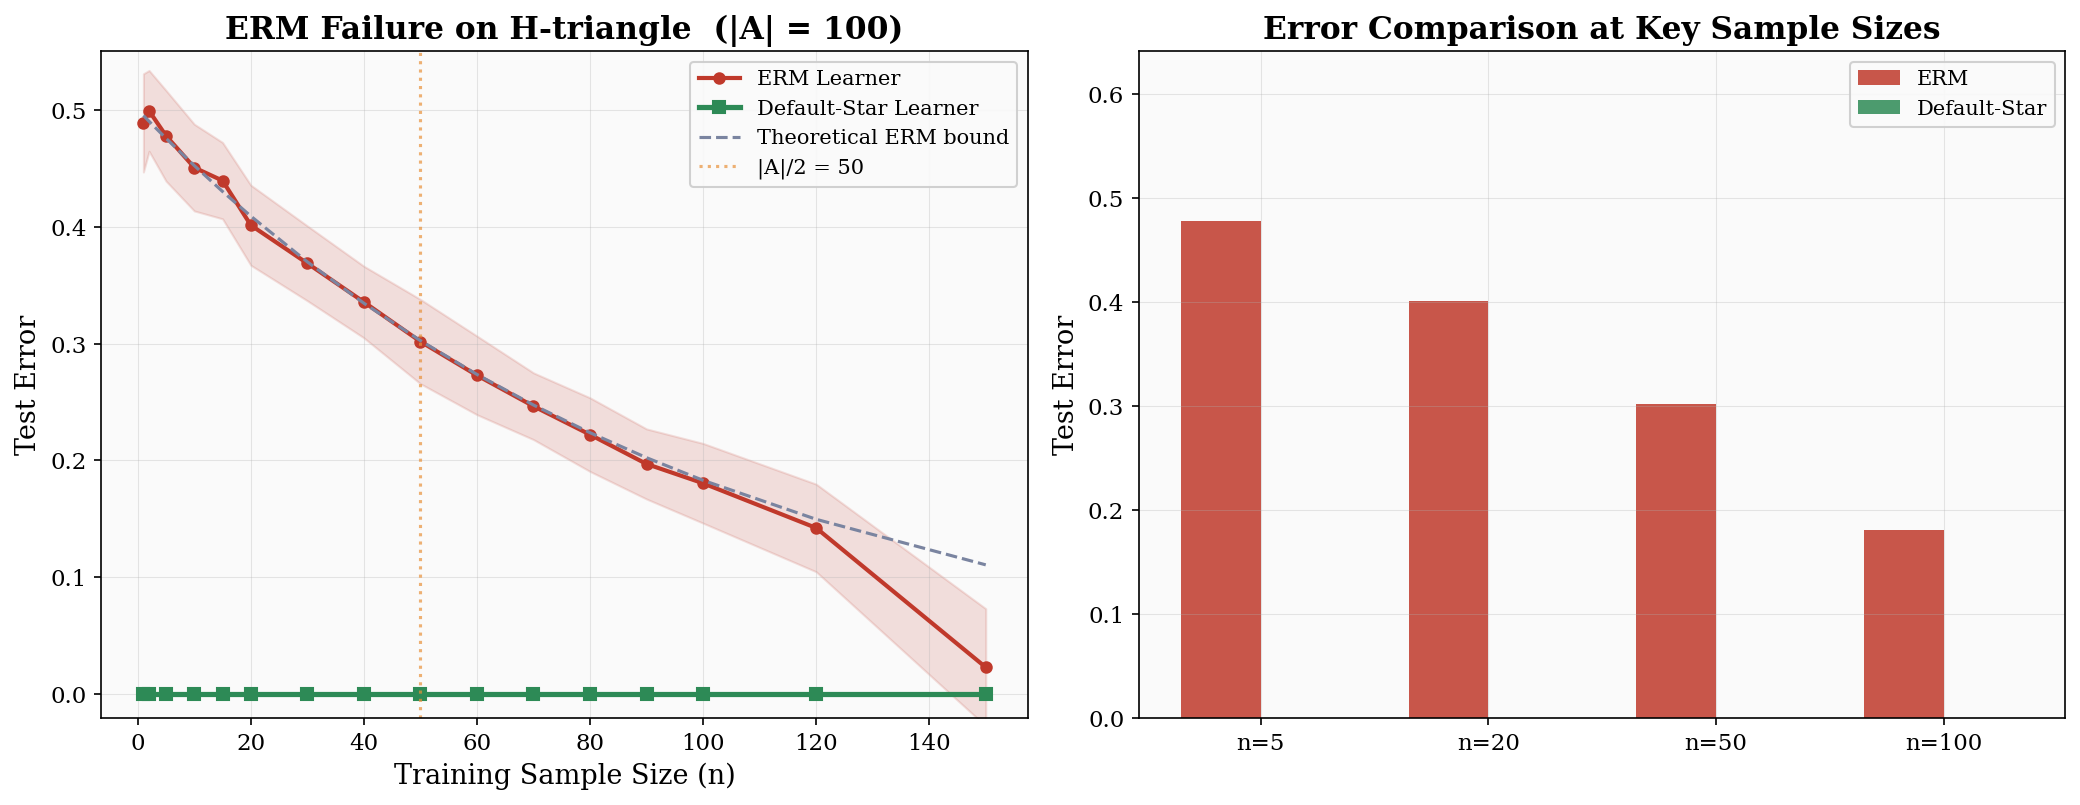
\includegraphics[width=\textwidth]{exp1_erm_failure.png}
    \caption{ERM (red) starts near 50\% error and declines slowly. Default-Star (green) is zero throughout. Dashed line = theoretical bound $(1-1/k)^n \cdot 0.5$. Right: bar chart at key sample sizes. ($|A|=100$)}
    \label{fig:erm}
\end{figure}

Figure~\ref{fig:erm} shows the core result. ERM has $\sim$48\% error at $n=5$ and still $\sim$18\% at $n=100$. The simulation matches the theoretical bound closely. Default-Star achieves zero error from the first sample because it immediately learns $A$ from any observed label.

\subsection{Experiment 2: Scaling with $|A|$}

\begin{figure}[h]
    \centering
    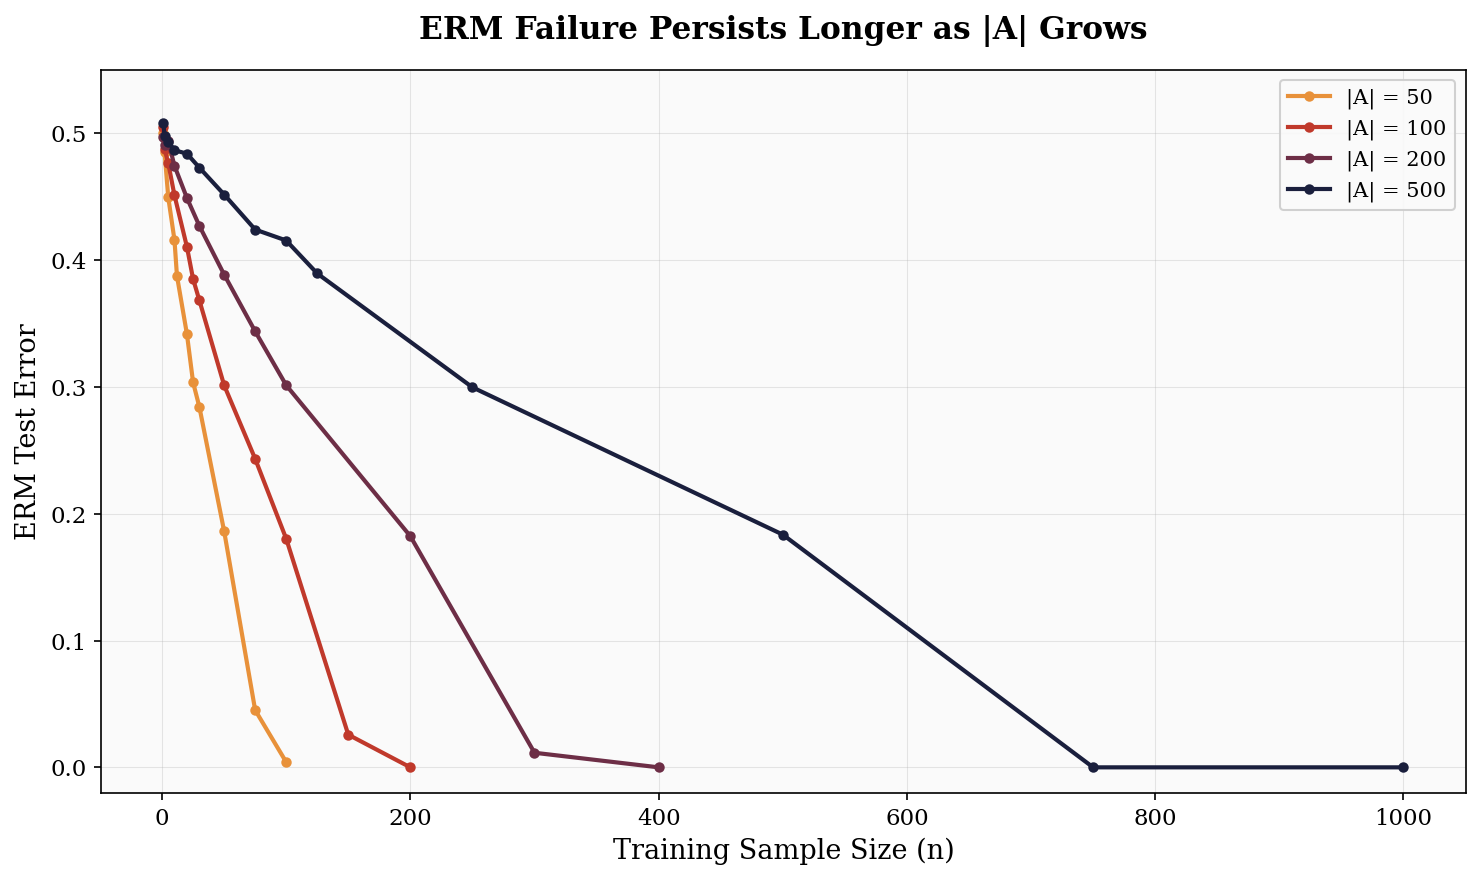
\includegraphics[width=0.75\textwidth]{exp2_scaling.png}
    \caption{ERM error for $|A| \in \{50, 100, 200, 500\}$. Larger sets = longer failure.}
    \label{fig:scale}
\end{figure}

Figure~\ref{fig:scale} confirms the paper's key theoretical point: as $|A|$ grows, ERM needs proportionally more samples. At $n = |A|/2$, all curves show $\sim$30\% error. For $|A|=500$, ERM still fails at $n=500$. This means ERM cannot learn $\mathcal{H}_\triangle$ with bounded sample complexity.

\subsection{Experiment 3: Local Regularization Strategies}

\begin{figure}[h]
    \centering
    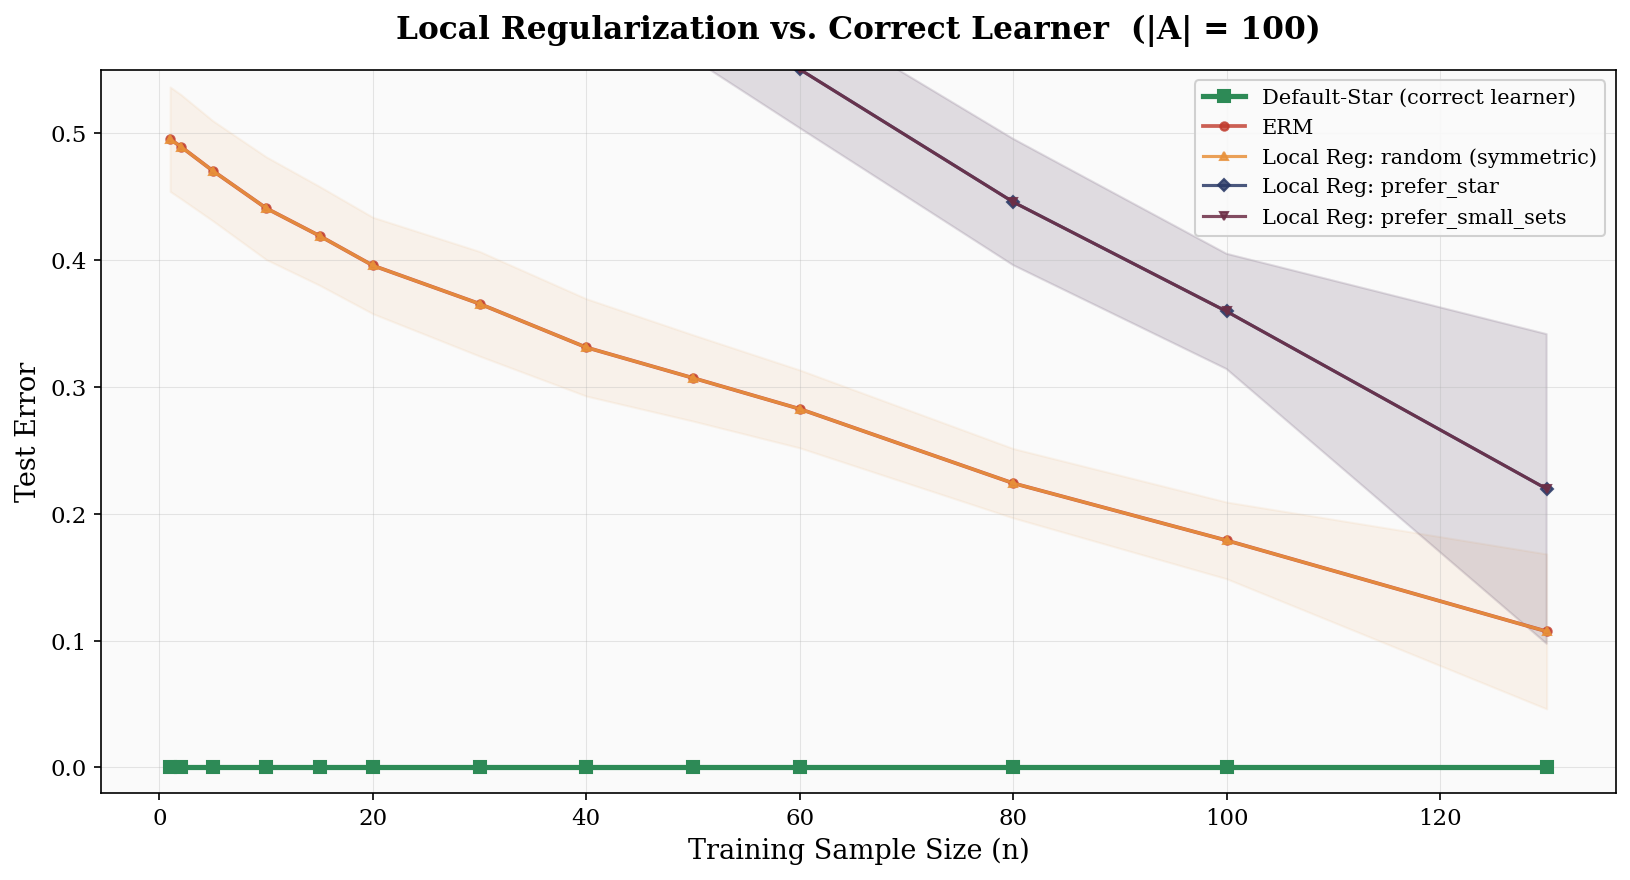
\includegraphics[width=0.8\textwidth]{exp3_local_reg_comparison.png}
    \caption{All local regularizer strategies fail. Random $\psi$ (orange) $\approx$ ERM. Prefer-star and prefer-small (blue, purple) are even worse. Default-Star (green) = zero.}
    \label{fig:localreg}
\end{figure}

Figure~\ref{fig:localreg} is the most important result for the open problem. Every $\psi$ strategy I tested fails:
\begin{itemize}[leftmargin=*,itemsep=1pt]
    \item \textbf{Random/symmetric}: identical to ERM --- no useful bias.
    \item \textbf{Prefer-star}: worse --- always predicts $*$ on unseen points, wrong whenever the true label is a set.
    \item \textbf{Prefer-small-sets}: also worse --- picks adversarial small set $B$ over correct large set $A$.
\end{itemize}
No strategy breaks the symmetry because $\psi(h, x)$ cannot access the training data.

\subsection{Experiment 4: Symmetry Visualization}

\begin{figure}[h]
    \centering
    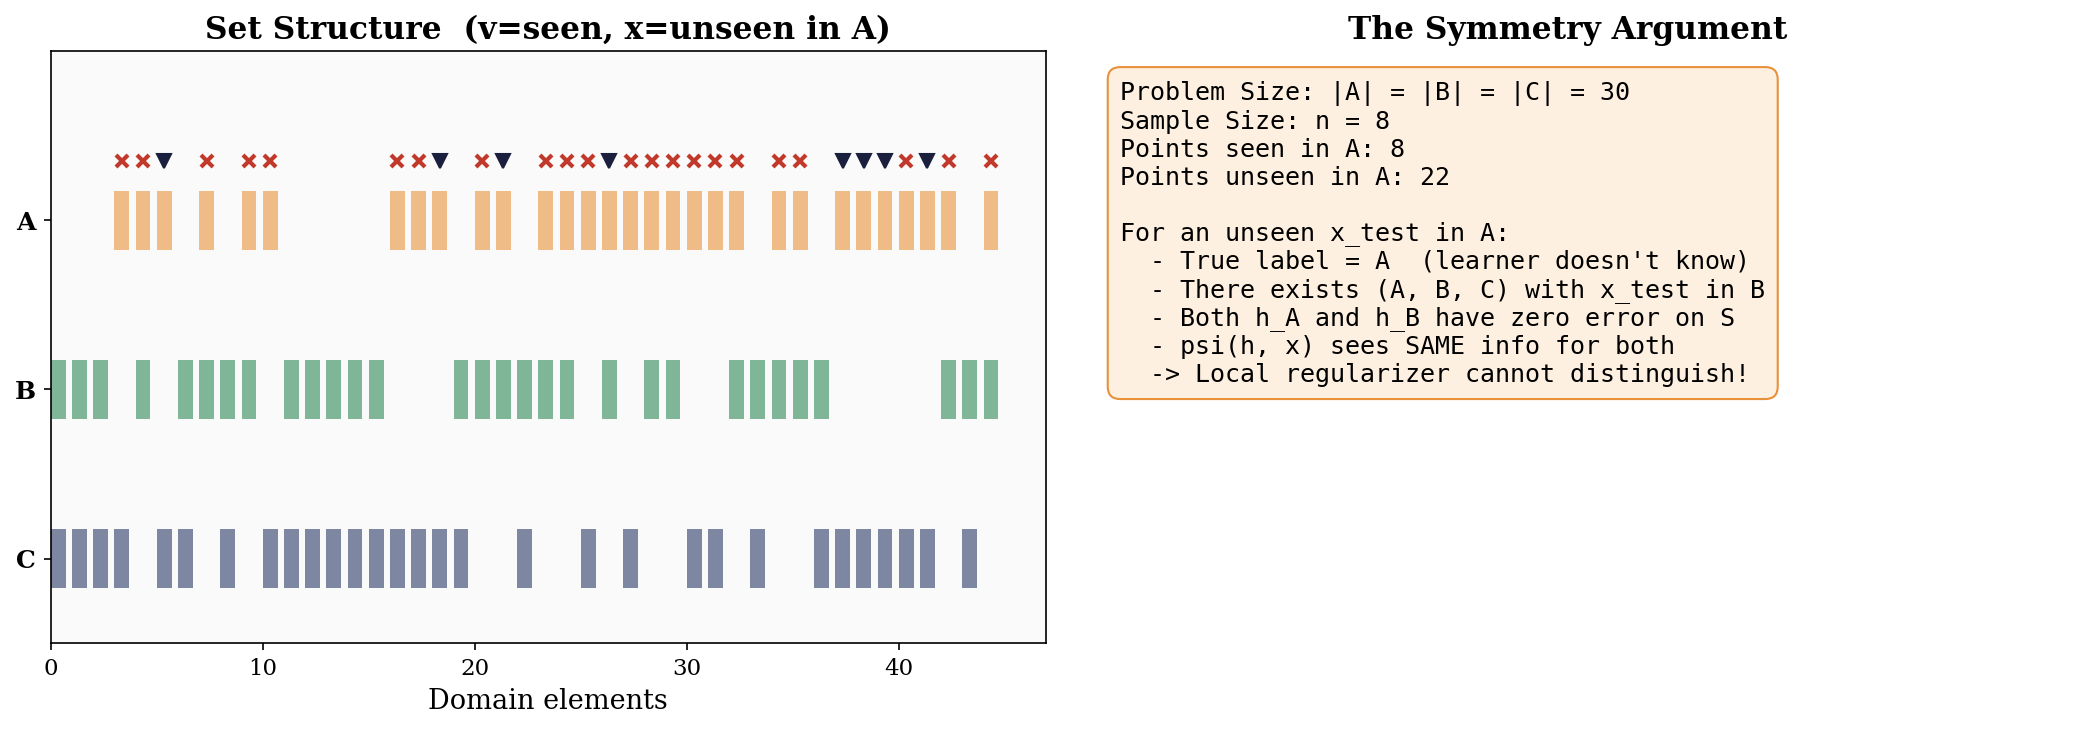
\includegraphics[width=\textwidth]{exp4_symmetry.png}
    \caption{Left: set structure (seen = $\blacktriangledown$, unseen = $\times$). Right: the symmetry argument --- $\psi(h,x)$ sees identical info for correct and adversarial hypotheses.}
    \label{fig:sym}
\end{figure}

Figure~\ref{fig:sym} visualizes \textit{why} local regularizers fail. For an unseen $x_{\text{test}} \in A$, an adversarial triple puts $x_{\text{test}}$ also in $B$. Both the correct hypothesis (predict $A$) and adversarial hypothesis (predict $B$) have zero training error. Since $\psi$ only sees $h$ and $x$---not the training sample---it gets the exact same information for both. There's no way to distinguish them.

\subsection{Experiment 5: Summary}

\begin{figure}[h]
    \centering
    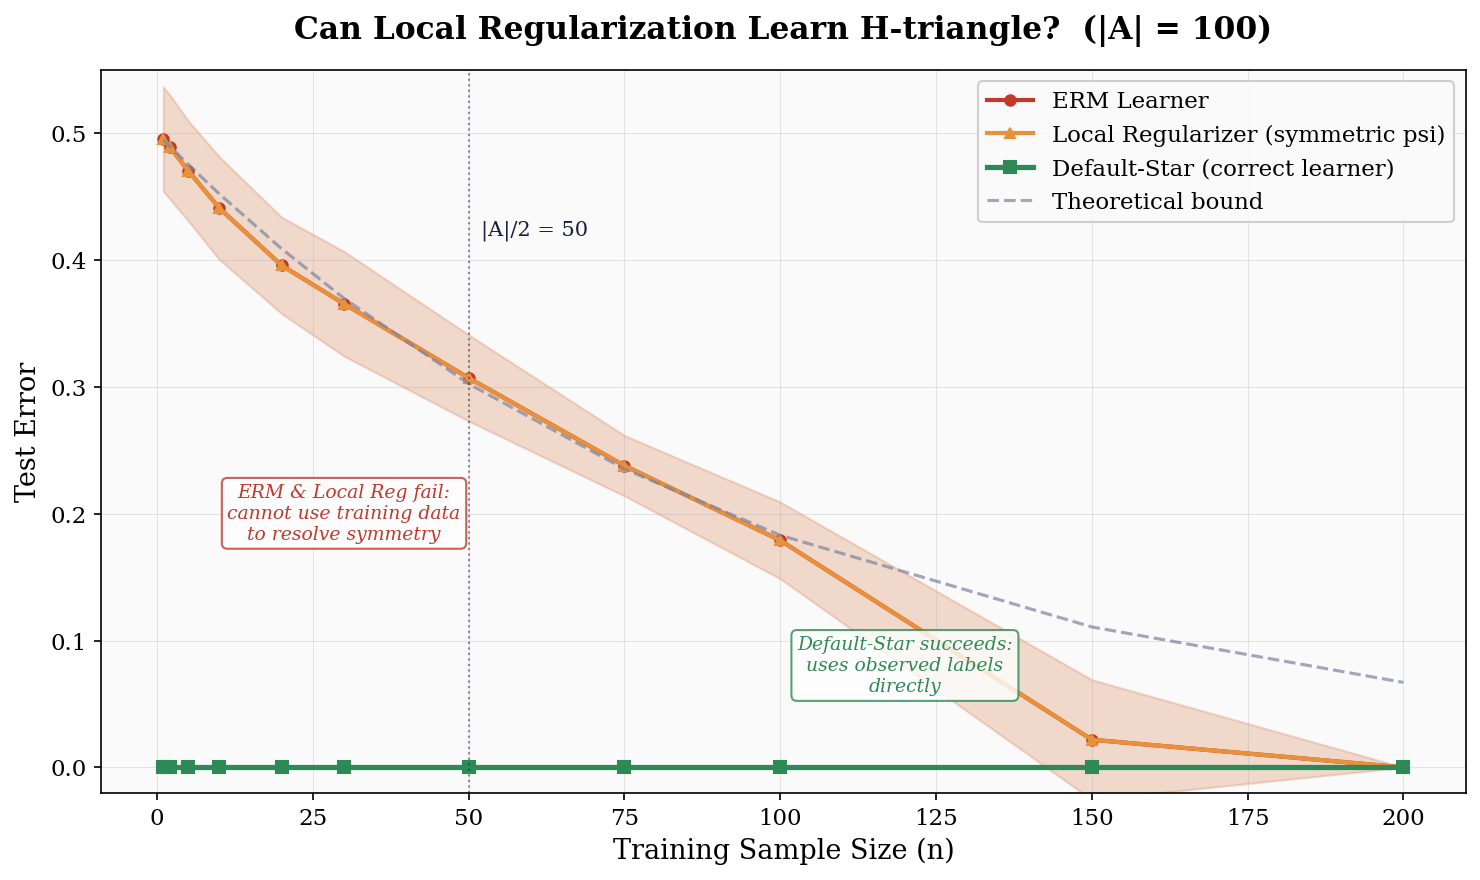
\includegraphics[width=0.8\textwidth]{exp5_summary.png}
    \caption{ERM (red) and local regularizer (orange) overlap. Theoretical bound (dashed) matches. Default-Star (green) = zero. ($|A|=100$)}
    \label{fig:summary}
\end{figure}

Figure~\ref{fig:summary} puts it all together. ERM and the symmetric local regularizer are nearly indistinguishable---both fail the same way because neither can use training data to resolve the symmetry. The theoretical bound matches the simulation. Default-Star succeeds because it uses observed labels directly.

\section{Discussion and Conclusion}

My experiments provide clear evidence that local regularization struggles on $\mathcal{H}_\triangle$. The root cause is the symmetry argument: $\psi(h,x)$ has no access to training data, so it cannot tell the correct label from an adversarial one. This supports the paper's conjecture toward a negative resolution of the open problem.

A few caveats: (1) this is empirical, not a formal proof; (2) I only tested a finite set of $\psi$ strategies---there could be a clever one I didn't try; (3) the unsupervised variant of local regularization (which CAN see unlabeled data) already works, so the gap is narrow.

If local regularization turns out to be insufficient, it means the training sample geometry is genuinely essential for multiclass learning, and the complex OIG-based learners are necessary. If sufficient, we'd get a clean, simple learning template for multiclass. Either way, the answer has significant implications for learning theory.

{\small
\bibliographystyle{plainnat}
\begin{thebibliography}{7}

\bibitem[Asilis et~al.(2024a)]{asilis2024}
Asilis, J., Devic, S., Dughmi, S., Sharan, V., and Teng, S.-H.
\newblock Regularization and optimal multiclass learning.
\newblock \emph{COLT}, 2024.

\bibitem[Asilis et~al.(2024b)]{asilis2024open}
Asilis, J., Devic, S., Dughmi, S., Sharan, V., and Teng, S.-H.
\newblock Open problem: Can local regularization learn all multiclass problems?
\newblock \emph{PMLR}, 196:1--5, 2024.

\bibitem[Brukhim et~al.(2022)]{brukhim2022}
Brukhim, N., Carmon, D., Dinur, I., Moran, S., and Yehudayoff, A.
\newblock A characterization of multiclass learnability.
\newblock \emph{FOCS}, 2022.

\bibitem[Daniely and Shalev-Shwartz(2014)]{daniely2014}
Daniely, A. and Shalev-Shwartz, S.
\newblock Optimal learners for multiclass problems.
\newblock \emph{COLT}, 2014.

\bibitem[David et~al.(2016)]{david2016}
David, O., Moran, S., and Yehudayoff, A.
\newblock On statistical learning via the lens of compression.
\newblock \emph{NeurIPS}, 2016.

\bibitem[Valiant(1984)]{valiant1984}
Valiant, L.~G.
\newblock A theory of the learnable.
\newblock \emph{Comm.\ ACM}, 27(11):1134--1142, 1984.

\bibitem[Vapnik and Chervonenkis(1971)]{vapnik1971}
Vapnik, V.~N. and Chervonenkis, A.~Ya.
\newblock On uniform convergence of relative frequencies of events to their probabilities.
\newblock \emph{Theory Prob.\ Appl.}, 16:264--280, 1971.

\end{thebibliography}
}

\end{document}
